\documentclass[tikz,border=2pt]{standalone}

\usepackage{pgfplots}
\usepackage{ctex}

\usepgfplotslibrary{}
\pgfplotsset{compat=1.18,width=4.5cm,height=6cm}
\usetikzlibrary{intersections,shapes.geometric,positioning,arrows.meta}

\begin{document}
	\begin{tikzpicture}
		\draw[-Stealth] (-1,0) -- (3,0)node[below]{$x$};
		\draw [-Stealth](0,-2.5) -- (0,1.4)node[left]{$y$};
		\draw[magenta] (0,0) -- +(-45:2.5)coordinate(a)circle(2pt);
		\draw[magenta,-{Stealth[length=2mm,width=1mm,inset=0.2mm]},dashed](a) -- +(0,0.5)coordinate(b);
		\draw[magenta,dashed] (b) -- (0,0);
		\node[below] at(a){热带风暴中心};
		\node(0,0)[above right=-3pt]{码头};
		\draw[magenta](0,-0.5) arc(-90:-45:0.5);
		\path (0,0) -- +(-88:0.5)node[below right=-3pt]{$45^\circ$};
	\end{tikzpicture}
	
	
\begin{tikzpicture}
		\draw[line width=8pt,draw=pink,fill=green!60!black](0,0) rectangle (2,1.5);
	\end{tikzpicture}
	
	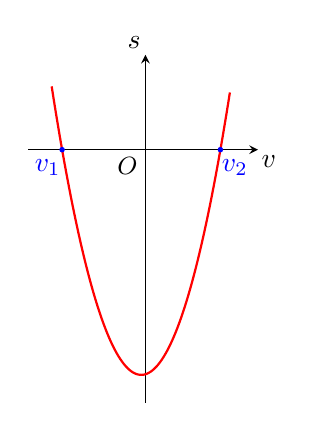
\begin{tikzpicture}
		\begin{axis}[%
			axis lines=center,
			no markers,
			xmin=-125,xmax=120,
			ymax=3000,ymin=-8000,		
%			xticklabels={0.2,0.4,0.6},
%			xtick={40,50,60},
%			extra x ticks={1/3},
%			extra x tick labels={$\frac{1}{3}$},
%			xtick distance=0.1,
%			ytick distance=0.1,
%			ytick={10,20,-20,-10},
%			yticklabels={0.2,0.4,0.6,0.8},
			xtick=\empty,ytick=\empty,
			yticklabel style={font=\small\rmfamily},
			xticklabel style={font=\small\rmfamily},
			ytick align=inside,
			major tick length=0.5mm, 
			yticklabel shift=-1mm,
			xticklabel shift=-1mm,
			ylabel=$s$,xlabel=$v$,
			xlabel shift=-1em,
			ylabel shift=1cm,
			xlabel style={xshift=1em,yshift=-1em},
			ylabel style={xshift=-1em,yshift=1em},
			declare function={
				f(\x) = (\x)^2 + 9*(\x) - 7100;
			},
			]
			\addplot+ [name path = curve,samples=100,red,thick,domain=-100:90]{f(x)};
			\path[name path = line](-200,0) -- (400,0);
			\fill[name intersections={of=line and curve,name=t},blue]
			(t-1)node[below left=0pt and -3pt,blue]{$v_1$}circle(1pt)
			(t-2)node[below right= 0pt and -3pt,blue]{$v_2$}circle(1pt);

			\node at(0,0) [below left=-1pt]{\small $O$};
%			\addplot[only marks,mark=*,mark size=1.5pt,magenta] 
%			coordinates {(50,0) 
%			(60,0)};
            \end{axis}
            
            
	\end{tikzpicture}
		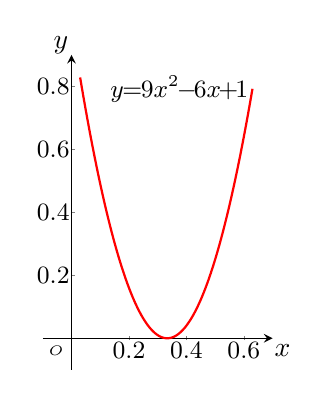
\begin{tikzpicture}
		\begin{axis}	[,axis lines=center,
			no markers,xmin=-0.1,xmax=0.7,
			ymax=0.9,ymin=-0.1,		
			xticklabels={0.2,0.4,0.6},
			xtick={0.2,0.4,0.6},
			xtick distance=0.1,
			ytick distance=0.1,
			ytick={0.2,0.4,0.6,0.8},
			yticklabels={0.2,0.4,0.6,0.8},
			yticklabel style={font=\small\rmfamily},
			xticklabel style={font=\small\rmfamily},
			ytick align=inside,
			y=4cm,
			major tick length=0.5mm, 
			,yticklabel shift=-1mm,
			xticklabel shift=-1mm,
			ylabel=$y$,xlabel=$x$,
			xlabel shift=-1em,
			ylabel shift=1cm,
			xlabel style={xshift=1em,yshift=-1em},
			ylabel style={xshift=-1em,yshift=1em},
			]
			\addplot+ [samples=100,domain=0.03:0.63,red,thick,]{9*x^2-6*x+1};
			\addplot[samples at={0.63}]{9*x^2-6*x+1}node[left=-2pt]{\small $y\!\!=\!\!9x^2\!\!-\!\!6x\!\!+\!\!1$};
			\node at(0,0) [below left=-1pt]{\tiny $O$};
		\end{axis}
		
		
	\end{tikzpicture}
	
	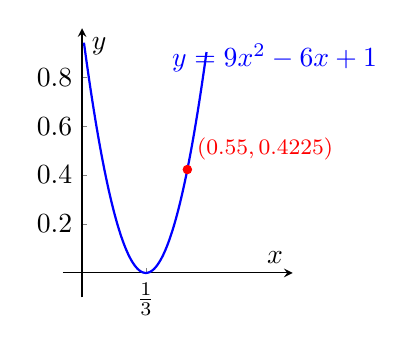
\begin{tikzpicture}
		\begin{axis}[
			width=4.5cm,
			height=5cm,
			axis lines=middle,          % 坐标轴在原点相交
			xlabel={$x$},
			ylabel={$y$},
			xmin=-0.1, xmax=1.1,
			ymin=-0.1, ymax=1.0,
			xtick={1/3},
			xticklabels={$\frac{1}{3}$},
			ytick={0,0.2,0.4,0.6,0.8},
			tick align=inside,
			axis line style={-stealth}, % 坐标轴带箭头
			enlargelimits=false,
			clip=false,
			samples=200,
			domain=0.01:0.65,
			major tick length=0.06cm,   % 主刻度线长度，默认 0.15cm
			minor tick length=0.04cm,   % 次要刻度线长度，默认 0.1cm
			]
			\addplot[blue, thick] {9*x^2 - 6*x + 1};
			\node[anchor=west, blue] at (axis cs:0.42, 0.88)
			{$y=9x^2-6x+1$};
			 % 绘制横坐标为 0.55 的点
			\addplot[only marks, mark=*, mark size=1.5pt, red]
			coordinates {(0.55, 0.4225)};
			
			% 可选：在该点旁边标注坐标
			\node[anchor=south west, red, font=\footnotesize]
			at (axis cs:0.55, 0.4225) {$(0.55,0.4225)$};
		\end{axis}
	\end{tikzpicture}
	
	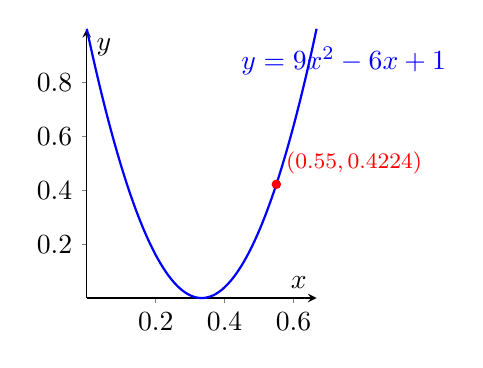
\begin{tikzpicture}
		
		\begin{axis}[
		width=4.5cm,
		height=5cm,
		axis lines=middle,
		xlabel={$x$},
		ylabel={$y$},
		xmin=0, xmax=0.6667,
		ymin=0, ymax=1.0,
		xtick={0,0.2,0.4,0.6},
		ytick={0,0.2,0.4,0.6,0.8},
		tick align=outside,
		major tick length=0.06cm,
		minor tick length=0.04cm,
		axis line style={-stealth},
		enlargelimits=false,
		clip=false,
		samples=300,
		domain=0:0.6667,
		% 自定义函数 f(x) = 9x^2 - 6x + 1
		declare function={
			f(\x) = 9*(\x)^2 - 6*(\x) + 1;
		},
		]
		% 绘制函数曲线
		\addplot[blue, thick] {f(x)};
		
		% 标注函数解析式
		\node[anchor=west, blue] at (axis cs:0.42, 0.88)
		{$y=9x^2-6x+1$};
		
		% 自动计算 x=0.55 处的函数值
		\pgfmathparse{f(0.55)}
		\let\yval\pgfmathresult
		
		% 绘制横坐标为 0.55 的点
		\addplot[only marks, mark=*, mark size=1.5pt, red]
		coordinates {(0.55, \yval)};
		
		% 在点旁标注坐标
		\node[anchor=south west, red, font=\footnotesize]
		at (axis cs:0.55, \yval) {$(0.55,\yval)$};
	\end{axis}
	\end{tikzpicture}
\end{document}